\documentclass[mathserif]{beamer}
\usepackage[orientation=ladnscape, size=a0, scale=1]{beamerposter}
\usetheme{MinimalistPoster}

% ----- DEFINE FONT & RELATED -----
\usepackage{anyfontsize}
\usepackage{ragged2e}

% ----- DEFINE MATHS & RELATED -----
\usepackage[euler-digits]{eulervm}
\DeclareMathOperator\atanh{atanh}

% ----- DEFINE TABLES & RELATED -----
\usepackage{tabularx}

% ----- DEFINE GRAPHICS -----
\usepackage{graphicx,mwe}
\usepackage{tikz}
\usepackage{wrapfig}
\usepackage{subfigure}
\usetikzlibrary{shapes}
\usetikzlibrary{positioning}
\usepackage{pgfplots}
%\usepackage{subcaption}

% ----- DEFINE COLORS -----
\usepackage{xcolor,colortbl}
\RequirePackage{LightPalette}

% ----- DEFINE REF ----- %
\usepackage[backend=bibtex, style=numeric, sorting=none, maxcitenames=1,
    maxbibnames=1,locallabelwidth]{biblatex}

\renewcommand{\bibfont}{\tiny}
\AtEveryBibitem{\clearfield{issn}}
\AtEveryCitekey{\clearfield{issn}}
\AtEveryBibitem{\clearfield{doi}}
\AtEveryCitekey{\clearfield{doi}}
\AtEveryBibitem{\clearfield{journal}}
\AtEveryCitekey{\clearfield{journal}}
\AtEveryBibitem{\clearfield{volume}}
\AtEveryCitekey{\clearfield{volume}}
\AtEveryBibitem{\clearfield{number}}
\AtEveryCitekey{\clearfield{number}}
\AtEveryBibitem{\clearfield{pages}}
\AtEveryCitekey{\clearfield{pages}}
\AtEveryBibitem{\clearfield{note}}
\AtEveryCitekey{\clearfield{note}}
\AtEveryBibitem{\clearfield{url}}
\AtEveryCitekey{\clearfield{url}}
\AtEveryBibitem{\clearfield{publisher}}
\AtEveryCitekey{\clearfield{publisher}}
\bibliography{NOBRefs}

% ----- OTHER PACKAGES -----
\usepackage{multicol}
\usepackage{multirow}
\usepackage{outlines}
\usepackage[absolute,overlay]{textpos}


% ----- CUSTOM FUNCTIONS -----

% ----- TITLE ----- %

\title{ In search of silent shipping}
%\author{M. Ishaq and  K. W. Lee}
\institute{\centering Centre for Fluids and Complex Systems, Coventry University}

% ----- LOGO ----- %
%\logo{
\includegraphics[height=7.5cm]{logo/cov_phoenix_right.pdf}}

% ----- DOCUMENT START ----- %
\begin{document}
\begin{frame}[t]{}
	\begin{columns}[T]
		\begin{column}{0.35\textwidth}
			\begin{block}{What is an MHD drive?}
				Magnetohydrodynamic (MHD) drive or thrusters utilises the interaction between electric and magnetic fields in electrically conductive liquid, such as seawater, to generate thrust \textbf{without any mechanical moving parts!}
			\end{block}
			\begin{block}{How does it work?}
				\begin{enumerate}
					\item The MHD drive operates on the simple application of the \textbf{Right-hand rule}:
					\begin{center}
						\begin{tikzpicture}
							\node (img1) at (0,0){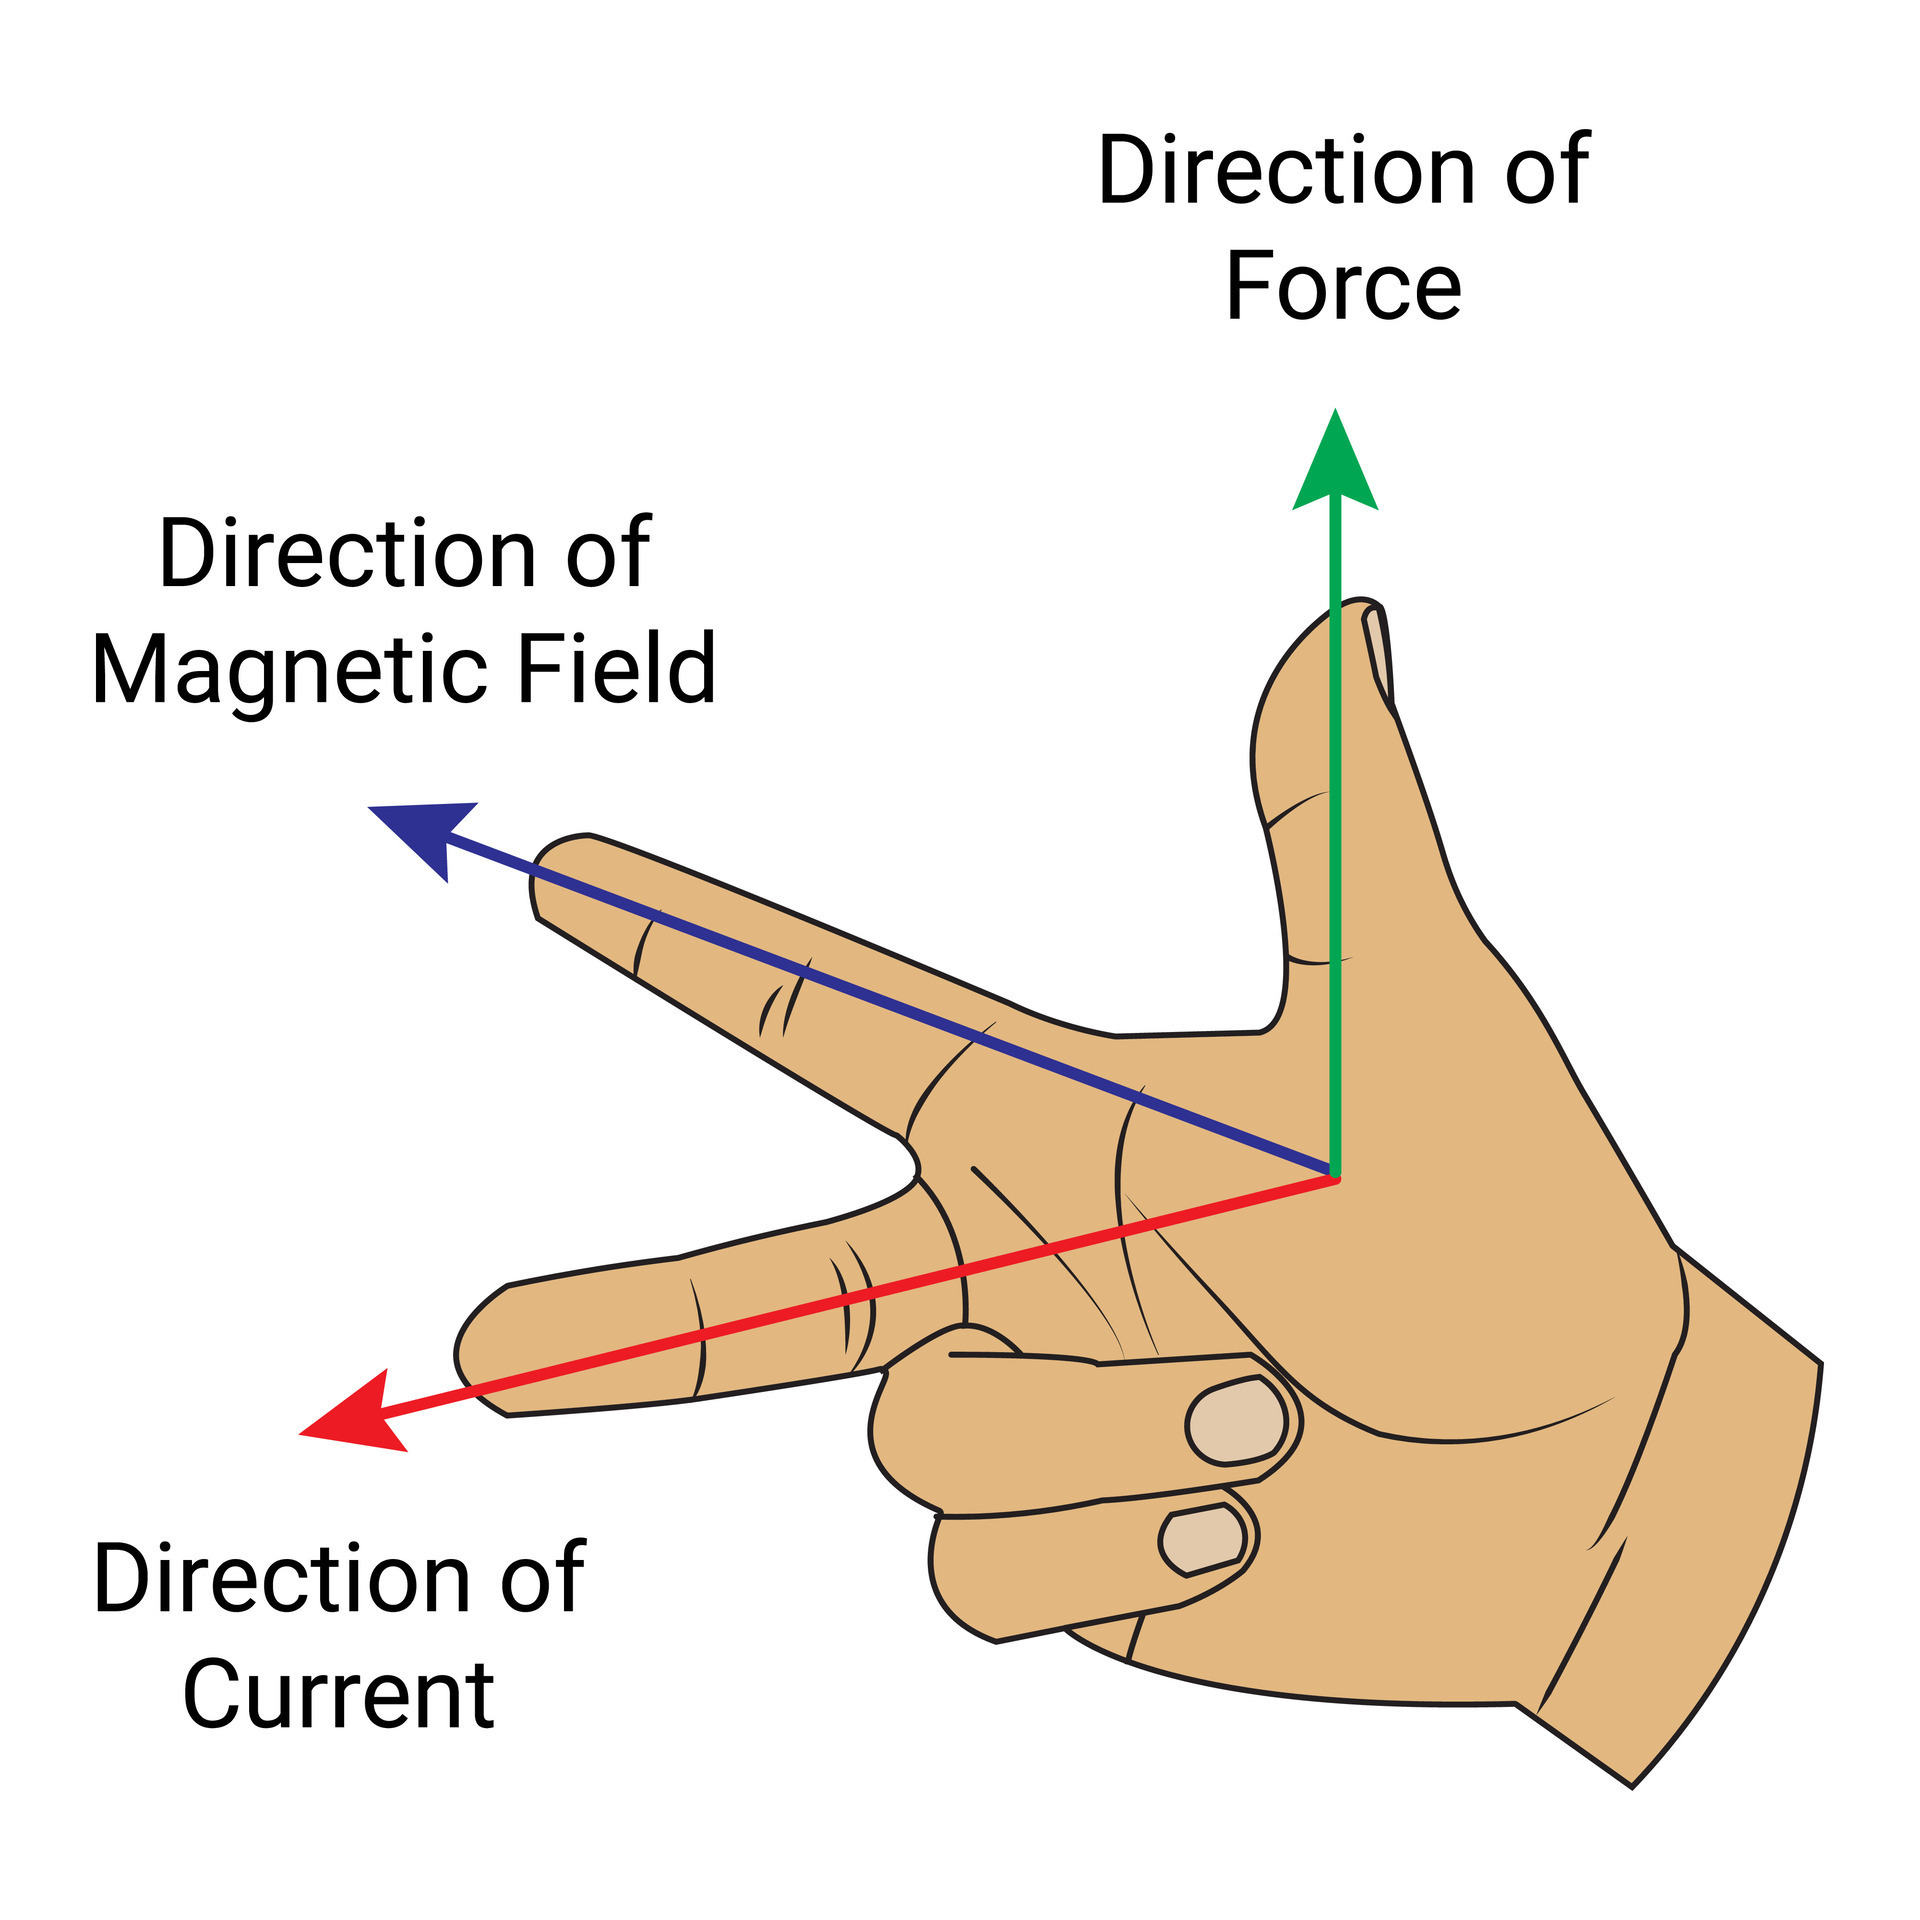
\includegraphics[width=0.4\textwidth]{img/righthandrule.png}};
						\end{tikzpicture} 
					\end{center}
					\item Seawater acts as an electrically conducting fluid. 
					\item By applying a strong magnetic field perpendicular to an electric field, an electromagnetic (Lorentz) force acts on electrical charges in seawater:
					\begin{center}
						\begin{tikzpicture}
							\node (img2) at (0,0){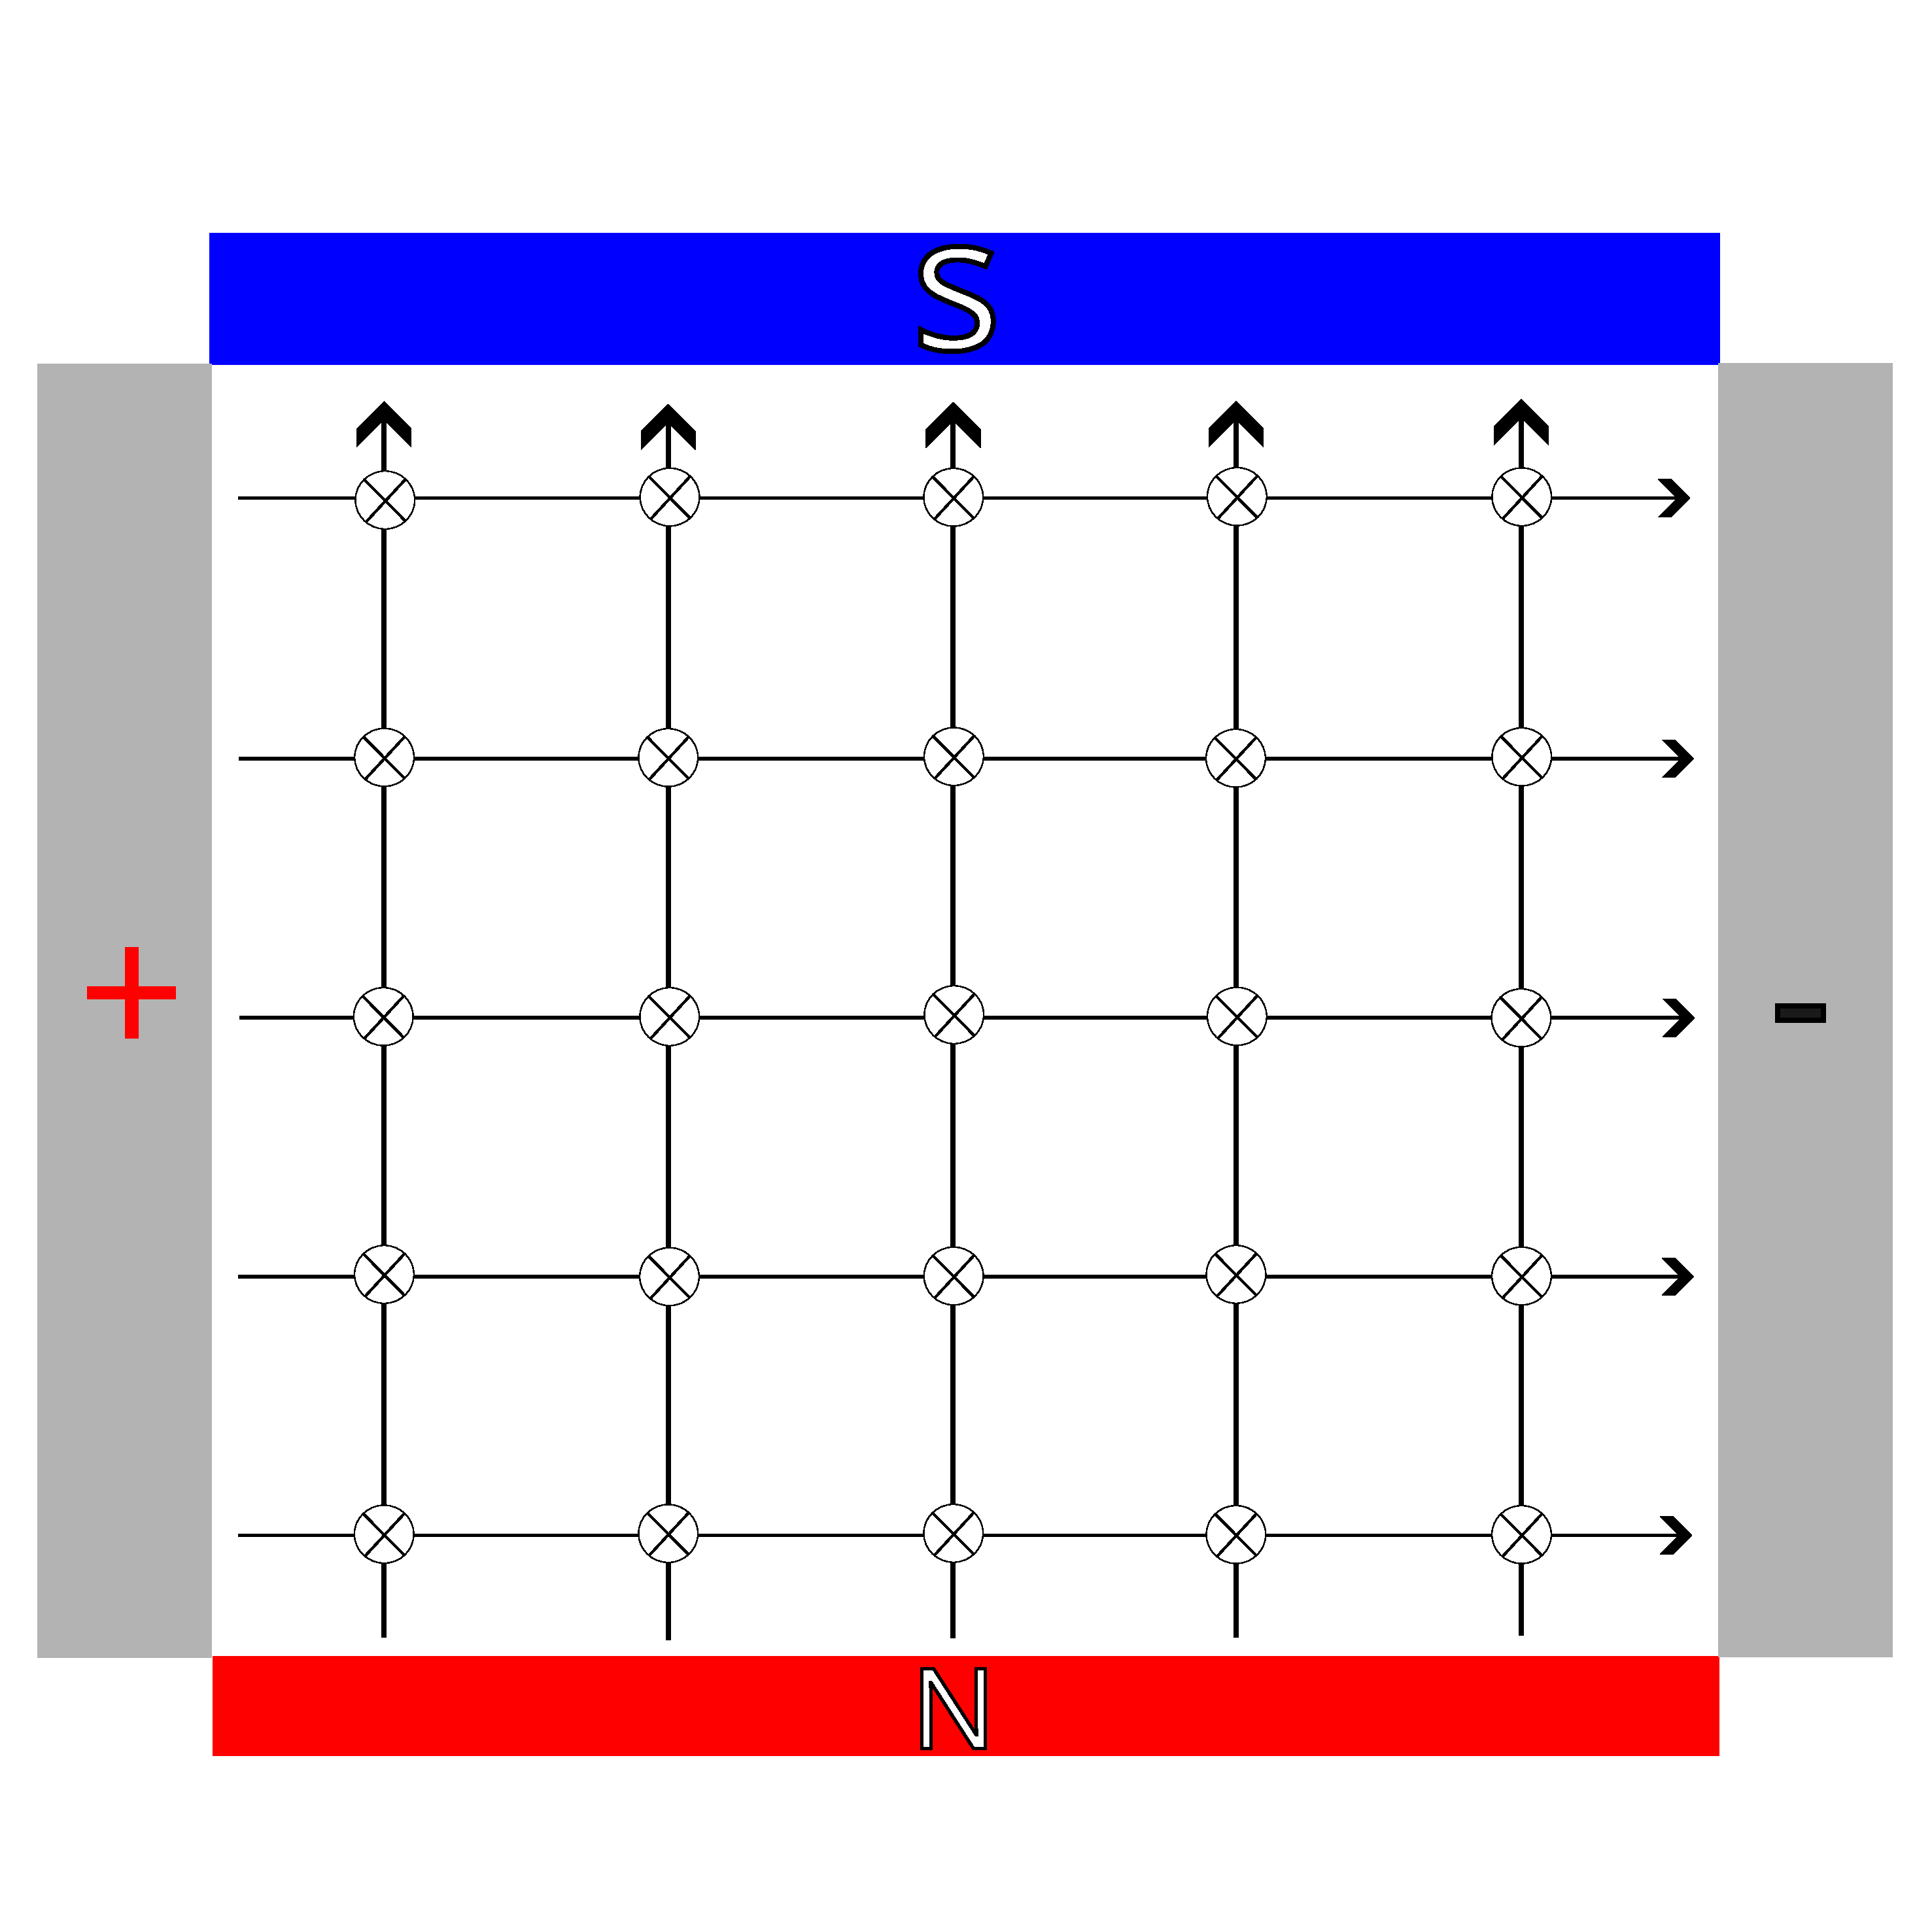
\includegraphics[width=0.4\textwidth]{svgs/thruster.pdf}};
						\end{tikzpicture}
					\end{center}					
					\item Mathematically, the Lorentz force is defined as:
						$$\overrightarrow {F} = \overrightarrow{J} \times \overrightarrow{B}$$
						
						 where $\overrightarrow{J}$ is the current density and $\overrightarrow{B}$ is the magnetic flux density.		
					\item Arranging the magnets and electrodes in a duct, we get the MHD thruster:
					\hfill \break
					\begin{center}
						\begin{tikzpicture}
							\node (img3) at (0,0){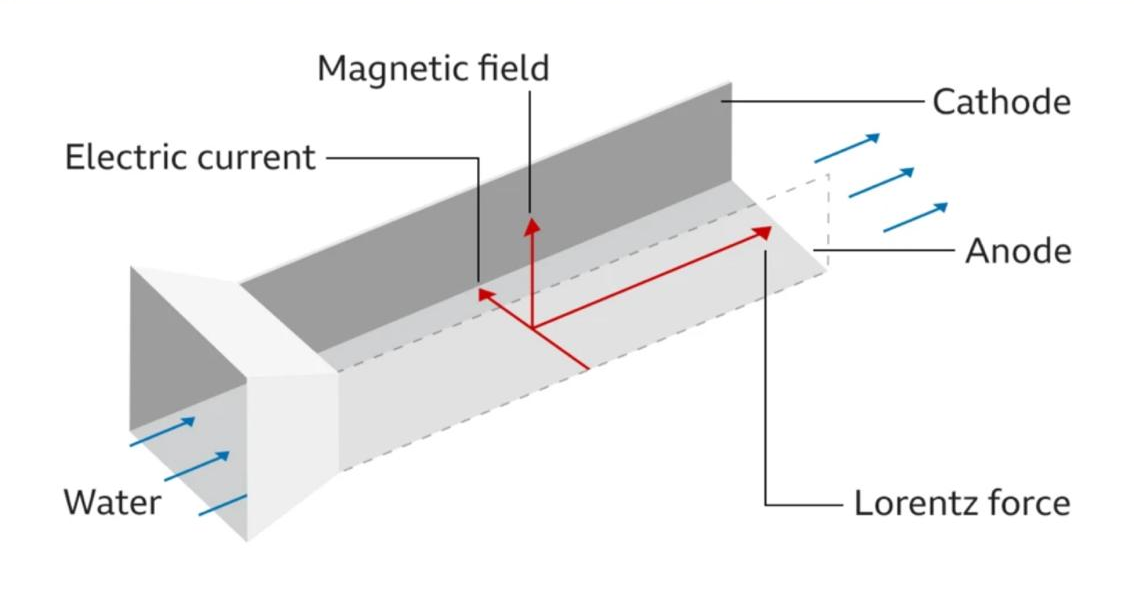
\includegraphics[width=0.5\textwidth]{img/thruster.png}};
						\end{tikzpicture}
					\end{center}
				\end{enumerate}
			\end{block}
		\end{column}
		\begin{column}{0.65\textwidth}
			\begin{block}{Why MHD drive?}
				
				\begin{center}
					\begin{tikzpicture}
						\node (img4) at (0,0){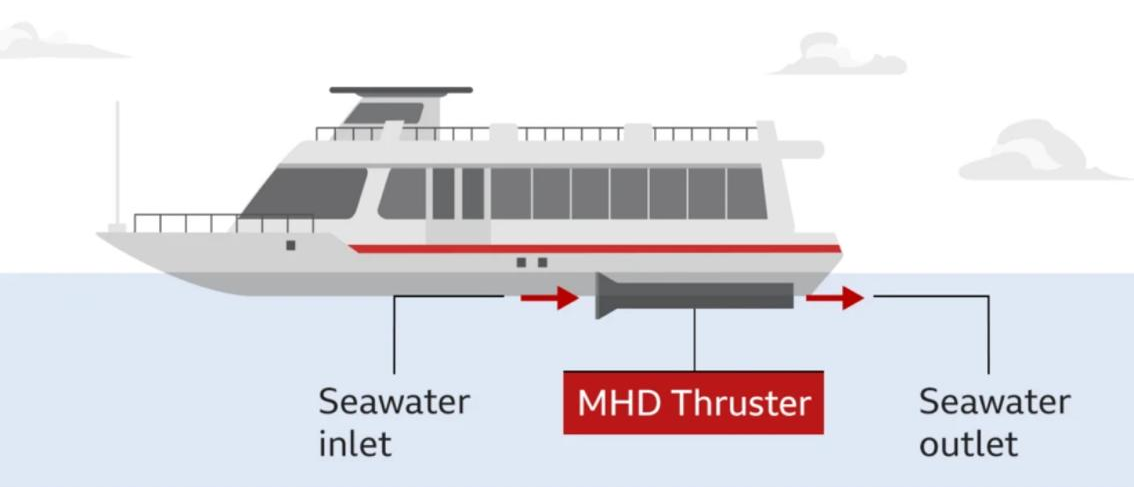
\includegraphics[width=0.4\textwidth]{img/BBCBoat.png}};
					\end{tikzpicture}
				\end{center}
				\begin{columns}[T]
					\begin{column}{0.5\textwidth}
				{\huge \textbf{Sustainability}:}
				\begin{outline}
					\1 Aquatic fauna that swim too close to propellers will be sucked in by the strong turbulence and sustain injury
					\1 Propeller-driven boats destroy aquatic flora in shallow waters (seagrass, corals, etc.)		
					\begin{center}
					\begin{tikzpicture}
						\node (img5) at (0.4\textwidth,0.1\textwidth){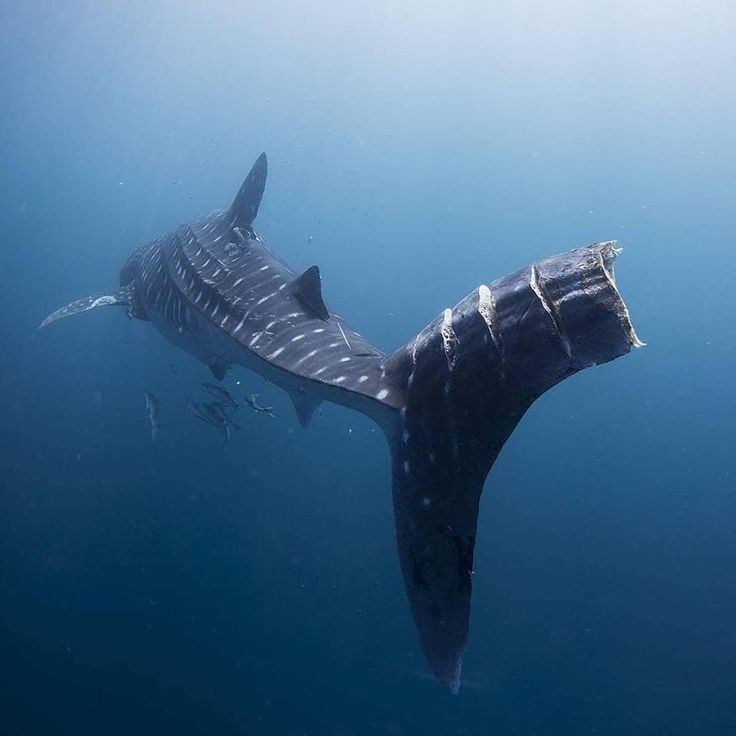
\includegraphics[width=0.4\textwidth]{img/scarring1.jpg}};
						\node (img6) at (0.0\textwidth,0){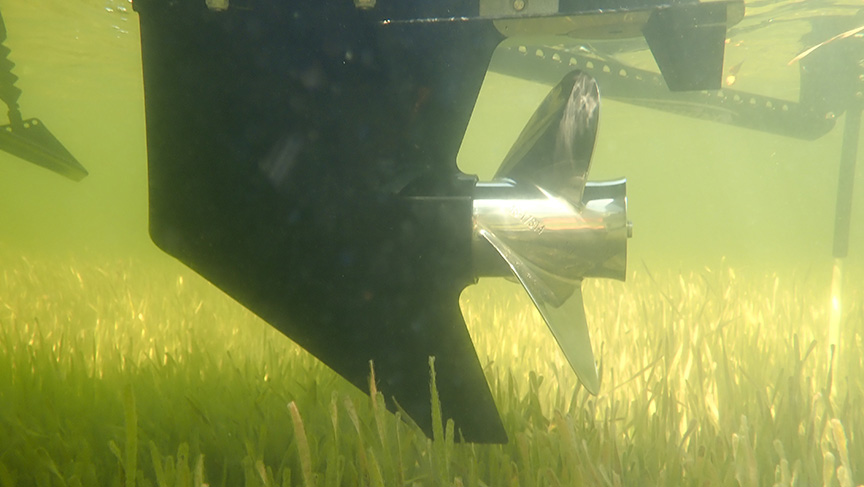
\includegraphics[width=0.35\textwidth]{img/seagrassscarring1.jpg}};
						\node (img7) at (0.0,0.2\textwidth){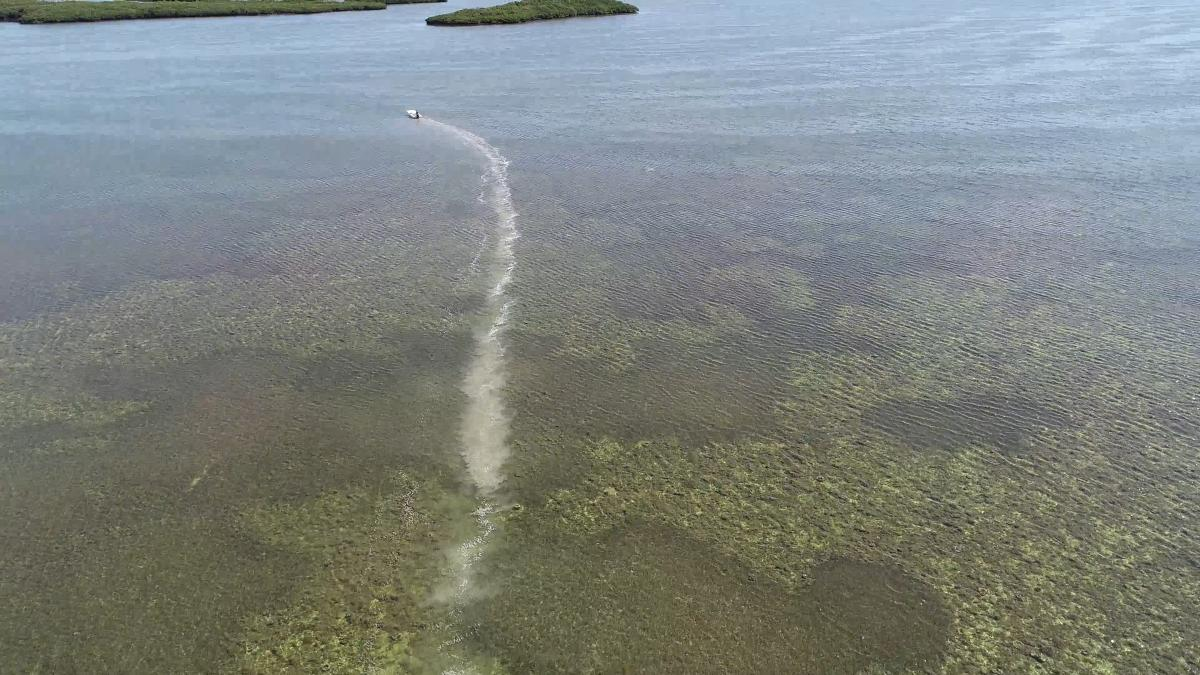
\includegraphics[width=0.35\textwidth]{img/seagrassscarring2.jpeg}};
					\end{tikzpicture}	
					\end{center}		
					\1 The lack of moving parts on MHD drive equipped ships will cause less damage to the environment
				\end{outline}
				\end{column}
				\begin{column}{0.5\textwidth}
				{\Huge \textbf{Revolutionising seacraft propulsion}:}
				\hfill \break
				\begin{outline}
					\1 Lack of moving parts reduces noise and vibration improves the stealth capabilities of submarines
					\begin{center}		
				\begin{tikzpicture}
					\node (yamato) at (0,0){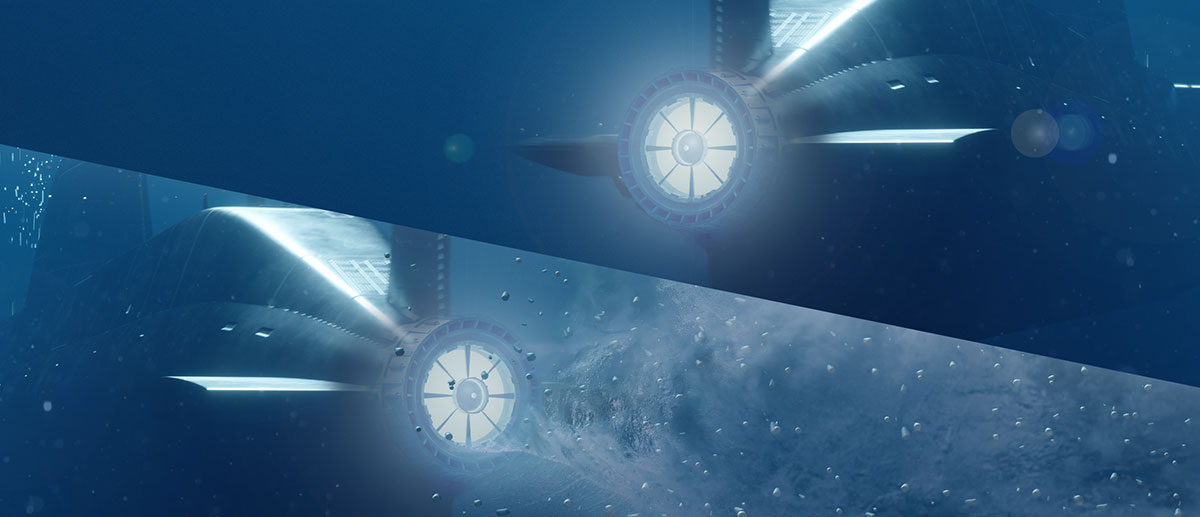
\includegraphics[width=0.8\textwidth]{img/PUMP-Press-Release.jpg}};
				\end{tikzpicture}
				\end{center}	
				\1 MHD drives can be made to exert force in any direction, improving manoeuvrability	
				\end{outline}				
				\end{column}
				\end{columns}
				\end{block}
				\begin{block}{The Skibidi Mk.I prototype}	
					\begin{center}		
				\begin{tikzpicture}
					\node (img1) at (0,0){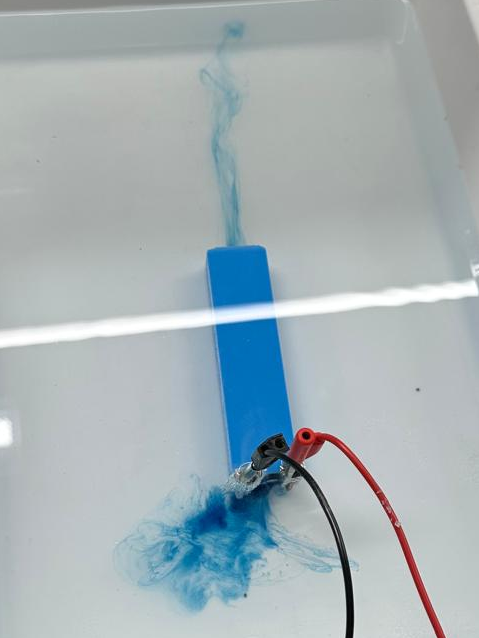
\includegraphics[width=0.15\textwidth]{img/thruster1.png}};
					\node [rotate=-90] (img2) at (0.25\textwidth,0){\includegraphics[width=0.21\textwidth]{img/2.jpg}};
					\node [rotate=-90] (img3) at (0.5\textwidth,0){\includegraphics[width=0.21\textwidth]{img/1.jpg}};
					\node [rotate=-90] (img4) at (0.75\textwidth,0){\includegraphics[width=0.21\textwidth]{img/3.jpg}};
				\end{tikzpicture}
				\end{center}
			\end{block}						
		\end{column}	
	\end{columns}
\end{frame}
\end{document}
